\section{Leiterplatten (PCBs)}
\subsection{Aufgaben Leiterplatte}
\begin{itemize}
  \item Gewährleistung der elektrischen Verbindungen zwischen den Bauelementen
  \item Mechanische Befestigung der Bauteile
  \item Wärmeabfuhr
  \item Ev. Abschirmfunktion
  \item Ev. Antennen (kleine Spulen)
\end{itemize}

\subsection{Eigenschaften Leiterplatte}
\begin{itemize}
  \item Die Leiterplatte ist ein zweidimensionaler Träger aus
  glasfaserverstärktem Polymer, in und auf dem Kupferbahnen und –flächen
  integriert sind.
  \item Spezifische elektrischen Eigenschaften:
  \begin{itemize}
    \item Die elektrischen Signale haben eine bestimmte, vom Material und den
    Abmessungen abhängige Signalgeschwindigkeit: die so genannte
    Phasengeschwindigkeit.
    \item Für schnelle Signale wird zusätzlich zur Ausbreitungsgeschwindigkeit
    die Wellenimpedanz wichtig.
    \item Die Isolationseigenschaften sind wichtig bei sehr kleinen Abständen
    zwischen den Leiterbahnen oder bei hohen Spannungsunterschieden.
    \item Für den Zusammenbau von ganzen Systemen sind die mechanischen
    Toleranzen und die kleinsten Abmessungen wichtig, welche hergestellt werden
    können.
    \end{itemize}
\end{itemize}

\subsection{Ausführungen}
\begin{itemize}
  \item Lagenzahl: - einlagig oder einseitig
  \item doppelseitig
  \item  Multilayer mit durchplattierten Vias
  \item  Multilayer mit Sackloch – Vias und Vias nur auf den Innenlagen
  \item Material: - starr, beispielsweise aus FR4
  \item Flex – Leiterplatte: stark elastisches Grundmaterial; damit kann sich
  die Leiterplatte an die Form des Gehäuses anpassen.
  \item Starr – Flex – Leiterplatte: Kombination aus Starr und Flex: die starren
  Zonen bieten den Bauteilen genügende mechanische Festigkeit, und die flexiblen
  Zonen bieten die Vorteile der Flexprints. (Erspart Connectors)
\end{itemize}

\subsection{Herausforderung Leiterplatten-Design}
\begin{itemize}
  \item Heute müssen vor der eigentlichen Layoutarbeit, schon bei der
  Konzipierung mit der Schaltungsentwicklung auch für die
  Leiterplattenherstellern und Baugruppenfertigung Technologien festgelegt und Absprachen getroffen werden, wovon immer auch das Design betroffen ist.
  \item Dessen Bearbeitung hat wiederum Einflüsse auf Schaltung und
  Fertigungsprozesse.
  \item Dies erfordert das Verständnis für die Tätigkeiten im
  Leiterplatten-Design
  \item \textbf{Design for Manufacturing}
  \item \textbf{Design for Environment}
  \item \textbf{Design for Recycling}
\end{itemize}

\subsection{Arbeitsablauf}
\begin{figure}[!htb]
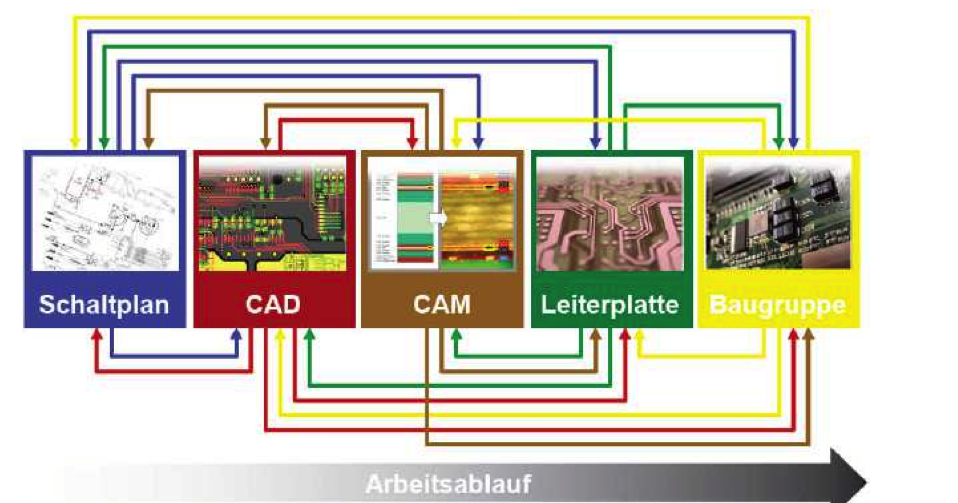
\includegraphics[scale=0.4]{pictures/arbeitsablauf}
\end{figure}

\subsection{Aufgaben Leiterplatten-Entwicklung}
\begin{multicols}{2}
\begin{itemize}
  \item Produktklassifizierung
  \item mechanische Gegebenheiten
  \item Einsatzumgebung
  \item Designrichtlinien
  \item Qualitätsrichtlinien
  \item EMV-Problematik
  \item thermische Gegebenheiten
  \item Bauteilekonfigurationen
  \item Leiterplattenmaterial
  \item Fertigungstechnologie
  \item Löt- und Befestigungstechnologie
  \item Bestückungstechnologie
  \item Testtechnologien
  \item Kosten- und Zeitfaktoren
  \item Reperaturmöglichkeiten
  \item Entsorgung und Umweltschutz
  \item Funktion
\end{itemize}
\end{multicols}

\subsection{Begriffe}
\begin{tabular}{p{6cm}p{11cm}}
\textbf{Via}:& Durchkontaktierung zwischen unterschiedlichen Lagen\\
\textbf{Buried Via (Vergrabene Durchkontaktierung)}: &In den Kernlagen liegende
  und aussen nicht sichtbare Durchkontaktierungen\\
\textbf{Blind Via (Sackloch)}: &Auf einer Innenlage endende Ankontaktierung.\\
\textbf{Microvia}: &An- oder Durchkontaktierung  mit einem Durchmesser unter 200
  $\mu$m\\
\textbf{SBU}:&Sequential Build Up\\
\textbf{HDI}:&High Density Interconnect\\
\end{tabular}
\begin{figure}[htb]
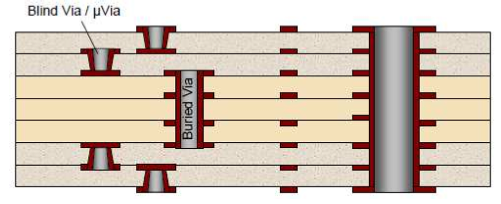
\includegraphics[scale=0.4]{pictures/begriffe}
\end{figure}

\subsection{High Speed Eigenschaften}
\begin{itemize}
  \item Kapazität und Induktivität von Vias
  \item C und L bei $\mu$Bia um ca. Faktor 10 kleiner (L=0,15 nH, C=0,04 pF)
  \item Geringere Impendanzsprung beim Layer-Wechsel
\end{itemize}

\begin{figure}[htb]
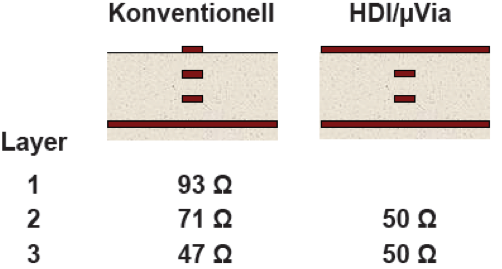
\includegraphics[scale=0.4]{pictures/highspeed}
\end{figure}

\subsection{Typischer Aufbau 4-Lagen}
\begin{tabular}{|l|l|l|l|}
\hline
Material&Lagen&Typ&Dicke[mm]\\
\hline
Cu-Folie&Lage 1&&0.018\\
\hline
Prepreg&&Prepreg 2116&0.115\\
\hline
Prepreg&&Prepreg 7628&0.180\\
\hline
Kupfer&Lage 2&&0.035\\
\hline
Innenlage&&FR4-Kern&0.9\\
\hline
Kupfer&Lage 3&&0.035\\
\hline
Prepreg&&Prepreg 7628&0.180\\
\hline
Prepreg&&Prepreg 2116&0.115\\
\hline
Cu-Folie&Lage 4&&0.018\\
\hline
\end{tabular}
\\
Theoretische Dicke ohne galvanisch Cu: 1.578 mm

\subsection{Herstellungsprozess}
\begin{itemize}
  \item Bohren
  \item Durchkontaktieren (bei doppelseitigen Leiterplatten)
  \item Fotoresist laminieren
  \item Belichten
  \item Entwickeln
  \item Ätzen
  \item Spülen 
  \item Trocknen
\end{itemize}

\subsection{Zusammenfassung}
\begin{itemize}
  \item Leiterplatten dienen der mechanischen Befestigung und der elektrischen
  Verbundung der Bauelemente
  \item Limiten des Leiterplatten-Design müssen schon bei der Entwicklung
  berücksichtigt werden
  \item Leiterplatten gibt es von 2 bis 24 Lagen
  \item Typische Leiterbahnbreite: 0.2mm, Abstand 0.25mm
  \begin{itemize}
    \item Kleinste Leiterbahnbreiten: 0.05mm
    \item Kupferdicke: Typ 35$\mu$m, auch 17$\mu$m
   \end{itemize}
\end{itemize}
